%% Research framework of the study (Figure 1). Compile with pdflatex; the manuscript
%% includes the resulting PDF (figures/fig_framework.pdf).
\documentclass[border=3pt]{standalone}
\usepackage{amsmath,amssymb}
\usepackage{tikz}
\usetikzlibrary{calc,arrows.meta,positioning,shadows.blur,shapes.arrows,backgrounds}
%% Simple vector icons drawn with TikZ primitives (original artwork, no external icon set).
%% Each icon fits roughly in [-0.5,0.5]^2; use  \pic[scale=..] at (x,y) {name=colour};
\tikzset{
  ic/.style={line width=0.6pt, line cap=round, line join=round},
  % ---- clipboard / survey
  pics/survey/.style={code={
    \draw[ic,#1,fill=#1!10,rounded corners=1.5pt] (-0.34,-0.46) rectangle (0.34,0.40);
    \draw[ic,#1,fill=#1!60,rounded corners=1pt] (-0.13,0.34) rectangle (0.13,0.48);
    \foreach \y in {0.18,-0.04,-0.26}{
      \draw[ic,#1] (-0.24,\y) -- (-0.18,\y-0.05) -- (-0.08,\y+0.06);
      \draw[ic,#1!70] (0.0,\y) -- (0.24,\y);}
  }},
  % ---- wind turbine
  pics/turbine/.style={code={
    \fill[#1!70] (-0.035,-0.5) -- (0.035,-0.5) -- (0.018,0.12) -- (-0.018,0.12) -- cycle;
    \foreach \a in {90,210,330}{
      \fill[#1,rotate around={\a:(0,0.14)}] (0,0.14) .. controls (0.05,0.24) and (0.04,0.40) .. (0,0.48)
            .. controls (-0.025,0.40) and (-0.03,0.24) .. (0,0.14);}
    \fill[white] (0,0.14) circle (0.035); \draw[ic,#1] (0,0.14) circle (0.035);
    \draw[ic,#1!60] (-0.3,-0.5) -- (0.3,-0.5);
  }},
  % ---- solar panel with sun
  pics/solar/.style={code={
    \fill[#1!15,draw=#1,ic] (-0.42,-0.30) -- (0.22,-0.30) -- (0.38,0.06) -- (-0.26,0.06) -- cycle;
    \foreach \t in {0.25,0.5,0.75}{
      \draw[#1,line width=0.4pt] ($(-0.42,-0.30)!\t!(0.22,-0.30)$) -- ($(-0.26,0.06)!\t!(0.38,0.06)$);}
    \draw[#1,line width=0.4pt] (-0.34,-0.12) -- (0.30,-0.12);
    \draw[ic,#1] (-0.05,-0.30) -- (-0.05,-0.46) (-0.18,-0.46) -- (0.08,-0.46);
    \fill[orange!90!yellow] (0.30,0.34) circle (0.09);
    \foreach \a in {0,45,...,315}{\draw[orange!90!yellow,line width=0.5pt] ($(0.30,0.34)+(\a:0.12)$) -- ($(0.30,0.34)+(\a:0.17)$);}
  }},
  % ---- factory with CO2 cloud
  pics/factory/.style={code={
    \fill[#1!15,draw=#1,ic] (-0.46,-0.46) -- (-0.46,-0.06) -- (-0.26,0.06) -- (-0.26,-0.06) -- (-0.06,0.06) -- (-0.06,-0.06)
          -- (0.14,0.06) -- (0.14,0.26) -- (0.26,0.26) -- (0.26,-0.46) -- cycle;
    \foreach \x in {-0.38,-0.20,-0.02}{\fill[#1!60] (\x,-0.30) rectangle (\x+0.09,-0.20);}
    \fill[gray!45] (0.22,0.34) circle (0.07) (0.32,0.40) circle (0.09) (0.44,0.36) circle (0.07) (0.33,0.30) circle (0.07);
    \node[font=\sffamily\bfseries,scale=0.32,text=black!70] at (0.33,0.36) {CO$_2$};
    \draw[ic,#1!60] (-0.5,-0.46) -- (0.34,-0.46);
  }},
  % ---- calendar
  pics/calendar/.style={code={
    \draw[ic,#1,fill=white,rounded corners=1.5pt] (-0.42,-0.42) rectangle (0.42,0.34);
    \fill[#1,rounded corners=1.5pt] (-0.42,0.16) rectangle (0.42,0.34);
    \foreach \x in {-0.22,0.22}{\draw[ic,#1!60!black,line width=1pt] (\x,0.28) -- (\x,0.44);}
    \foreach \i in {0,...,3}{\foreach \j in {0,1,2}{
      \pgfmathsetmacro{\px}{-0.27+\i*0.18}\pgfmathsetmacro{\py}{0.02-\j*0.15}
      \fill[#1!30] (\px,\py) circle (0.045);}}
    \foreach \i/\j in {0/0,2/0,0/2,2/2}{\pgfmathsetmacro{\px}{-0.27+\i*0.18}\pgfmathsetmacro{\py}{0.02-\j*0.15}
      \fill[#1] (\px,\py) circle (0.05);}
  }},
  % ---- gauge (normalisation)
  pics/gauge/.style={code={
    \fill[#1!12] (-0.44,-0.18) arc (180:0:0.44) -- cycle;
    \draw[ic,#1,line width=1.4pt] (-0.44,-0.18) arc (180:0:0.44);
    \foreach \a in {180,150,...,0}{\draw[#1,line width=0.5pt] ($(0,-0.18)+(\a:0.34)$) -- ($(0,-0.18)+(\a:0.42)$);}
    \draw[ic,black!75,line width=0.9pt] (0,-0.18) -- ++(55:0.34);
    \fill[black!75] (0,-0.18) circle (0.05);
    \node[font=\sffamily,scale=0.35] at (-0.38,-0.30) {0}; \node[font=\sffamily,scale=0.35] at (0.38,-0.30) {1};
  }},
  % ---- balance scale (weights)
  pics/balance/.style={code={
    \draw[ic,#1,line width=1pt] (0,-0.42) -- (0,0.34); \draw[ic,#1,line width=1pt] (-0.18,-0.44) -- (0.18,-0.44);
    \draw[ic,#1,line width=1pt,rotate around={-8:(0,0.28)}] (-0.40,0.28) -- (0.40,0.28);
    \fill[#1] (0,0.34) circle (0.045);
    \begin{scope}[rotate around={-8:(0,0.28)}]
      \draw[ic,#1] (-0.40,0.28) -- (-0.50,0.02) (-0.40,0.28) -- (-0.30,0.02);
      \fill[#1!30,draw=#1,ic] (-0.52,0.02) arc (180:360:0.12 and 0.07) -- cycle;
      \draw[ic,#1] (0.40,0.28) -- (0.30,0.02) (0.40,0.28) -- (0.50,0.02);
      \fill[#1!30,draw=#1,ic] (0.28,0.02) arc (180:360:0.12 and 0.07) -- cycle;
    \end{scope}
  }},
  % ---- podium
  pics/podium/.style={code={
    \fill[#1] (-0.14,-0.44) rectangle (0.14,0.10); \fill[#1!65] (-0.44,-0.44) rectangle (-0.14,-0.08);
    \fill[#1!40] (0.14,-0.44) rectangle (0.44,-0.18);
    \node[font=\sffamily\bfseries,white,scale=0.55] at (0,-0.10) {1};
    \node[font=\sffamily\bfseries,white,scale=0.5] at (-0.29,-0.25) {2};
    \node[font=\sffamily\bfseries,white,scale=0.5] at (0.29,-0.31) {3};
    \fill[orange!90!yellow] (0,0.30) -- (0.045,0.22) -- (0.13,0.21) -- (0.065,0.15) -- (0.08,0.06) -- (0,0.105)
          -- (-0.08,0.06) -- (-0.065,0.15) -- (-0.13,0.21) -- (-0.045,0.22) -- cycle;
  }},
  % ---- globe
  pics/globe/.style={code={
    \fill[#1!12] (0,0) circle (0.44); \draw[ic,#1] (0,0) circle (0.44);
    \draw[ic,#1] (0,-0.44) arc (-90:90:0.18 and 0.44) (0,-0.44) arc (270:90:0.18 and 0.44) (0,-0.44) -- (0,0.44);
    \draw[ic,#1] (-0.44,0) -- (0.44,0); \draw[ic,#1] (-0.39,0.2) -- (0.39,0.2) (-0.39,-0.2) -- (0.39,-0.2);
  }},
  % ---- shield with check
  pics/shield/.style={code={
    \fill[#1!15,draw=#1,ic] (0,0.46) -- (0.38,0.32) -- (0.36,-0.05) .. controls (0.30,-0.30) and (0.12,-0.40) .. (0,-0.47)
          .. controls (-0.12,-0.40) and (-0.30,-0.30) .. (-0.36,-0.05) -- (-0.38,0.32) -- cycle;
    \draw[ic,#1,line width=1.3pt] (-0.16,0.0) -- (-0.04,-0.13) -- (0.18,0.14);
  }},
  % ---- magnifier
  pics/magnifier/.style={code={
    \fill[#1!12] (-0.08,0.08) circle (0.28); \draw[ic,#1,line width=1.3pt] (-0.08,0.08) circle (0.28);
    \draw[#1,line width=3pt,line cap=round] (0.13,-0.13) -- (0.40,-0.40);
    \draw[ic,#1!70] (-0.22,0.02) -- (-0.14,0.14) -- (-0.04,0.06) -- (0.06,0.20);
  }},
  % ---- dice
  pics/dice/.style={code={
    \fill[#1!12,draw=#1,ic,rounded corners=3pt] (-0.40,-0.40) rectangle (0.40,0.40);
    \foreach \p in {(-0.2,0.2),(0.2,0.2),(0,0),(-0.2,-0.2),(0.2,-0.2)}{\fill[#1] \p circle (0.065);}
  }},
  % ---- target
  pics/target/.style={code={
    \fill[#1!12,draw=#1,ic] (0,0) circle (0.44); \fill[#1!35,draw=#1,ic] (0,0) circle (0.31);
    \fill[#1!12,draw=#1,ic] (0,0) circle (0.18);
    \fill[#1] (0,0) circle (0.07);
    \draw[ic,black!75,line width=0.9pt,-{Stealth[length=3pt]}] (0.46,0.46) -- (0.06,0.06);
  }},
  % ---- light bulb
  pics/bulb/.style={code={
    \fill[#1!15,draw=#1,ic] (-0.10,-0.18) .. controls (-0.12,-0.02) and (-0.28,0.04) .. (-0.28,0.18) arc (180:0:0.28)
          .. controls (0.28,0.04) and (0.12,-0.02) .. (0.10,-0.18) -- cycle;
    \fill[#1!70] (-0.11,-0.22) rectangle (0.11,-0.30); \fill[#1!70] (-0.09,-0.33) rectangle (0.09,-0.40);
    \draw[ic,#1] (-0.06,-0.18) -- (-0.04,0.10) -- (0,0.04) -- (0.04,0.10) -- (0.06,-0.18);
    \foreach \a in {20,55,90,125,160}{\draw[ic,orange!90!yellow] ($(0,0.18)+(\a:0.36)$) -- ($(0,0.18)+(\a:0.46)$);}
  }},
  % ---- document (literature)
  pics/document/.style={code={
    \fill[white,draw=#1,ic] (-0.32,-0.44) -- (-0.32,0.44) -- (0.16,0.44) -- (0.32,0.28) -- (0.32,-0.44) -- cycle;
    \fill[#1!30,draw=#1,ic] (0.16,0.44) -- (0.16,0.28) -- (0.32,0.28) -- cycle;
    \foreach \y in {0.22,0.08,-0.06,-0.20,-0.34}{\draw[ic,#1!70] (-0.22,\y) -- (0.22,\y);}
  }},
  % ---- speech bubble with question mark
  pics/question/.style={code={
    \fill[#1!15,draw=#1,ic,rounded corners=4pt] (-0.44,-0.22) rectangle (0.44,0.42);
    \fill[#1!15,draw=#1,ic] (-0.20,-0.215) -- (-0.30,-0.44) -- (-0.02,-0.215);
    \node[font=\sffamily\bfseries,text=#1,scale=0.9] at (0,0.10) {?};
  }},
  % ---- gear
  pics/gear/.style={code={
    \foreach \a in {0,45,...,315}{\fill[#1,rotate=\a] (-0.07,0.30) rectangle (0.07,0.44);}
    \fill[#1] (0,0) circle (0.33); \fill[white] (0,0) circle (0.13);
  }},
}

\definecolor{cData}{HTML}{16877F}
\definecolor{cProc}{HTML}{3B5BA5}
\definecolor{cWeight}{HTML}{D08414}
\definecolor{cRank}{HTML}{2E8B57}
\definecolor{cTrust}{HTML}{C0503F}
\definecolor{cOut}{HTML}{6B4FA0}
\definecolor{cInk}{HTML}{2D3748}
\definecolor{cSoft}{HTML}{F4F6F9}
\newcommand{\figtiny}{\fontsize{6}{7}\selectfont}
\begin{document}
\sffamily\hyphenpenalty=10000\exhyphenpenalty=10000
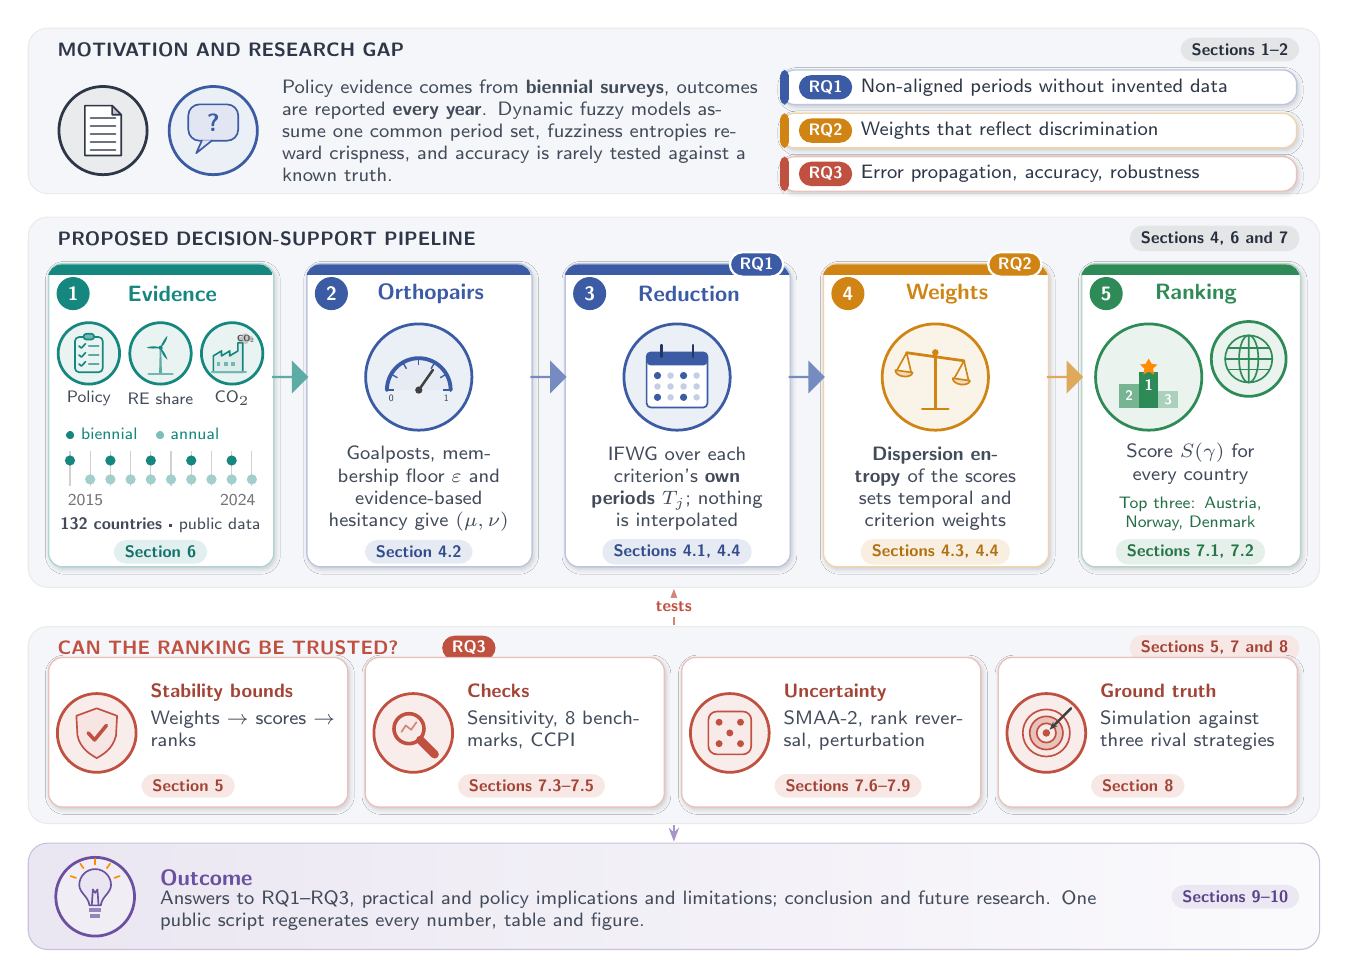
\begin{tikzpicture}[
  font=\sffamily\scriptsize, text=cInk,
  panel/.style={fill=cSoft, rounded corners=7pt, draw=black!8},
  card/.style={fill=white, rounded corners=5pt, draw=#1!35, line width=0.5pt,
               blur shadow={shadow blur steps=6, shadow xshift=0.6pt, shadow yshift=-0.9pt, shadow opacity=18}},
  topbar/.style={fill=#1, rounded corners=5pt},
  badge/.style={circle, fill=#1!10, draw=#1, line width=1pt, minimum size=1.12cm, inner sep=0pt},
  stepno/.style={circle, fill=#1, text=white, font=\sffamily\bfseries\scriptsize, minimum size=0.42cm, inner sep=0pt},
  ttl/.style={font=\sffamily\bfseries\footnotesize, text=#1, align=center},
  txt/.style={align=center, text width=#1, font=\sffamily\scriptsize, text=cInk!90},
  pill/.style={fill=#1!13, text=#1!85!black, font=\sffamily\bfseries\figtiny, rounded corners=4.5pt,
               inner xsep=4pt, inner ysep=2.2pt},
  rq/.style={fill=#1, text=white, font=\sffamily\bfseries\figtiny, rounded corners=4.5pt, inner xsep=3.5pt, inner ysep=2pt},
  chev/.style={single arrow, fill=#1, minimum height=0.46cm, minimum width=0.42cm,
               single arrow head extend=0.10cm, inner sep=0pt},
  band/.style={font=\sffamily\bfseries\scriptsize, text=#1, anchor=west},
]
%% ============================================================ 1. motivation
\fill[panel] (0,9.05) rectangle (16.4,11.15);
\node[band=cInk] at (0.25,10.88) {\MakeUppercase{Motivation and research gap}};
\node[pill=cInk, anchor=east] at (16.15,10.88) {Sections 1--2};
\node[badge=cInk] at (0.95,9.85) {}; \pic[scale=0.72] at (0.95,9.85) {document=cInk};
\node[badge=cProc] at (2.35,9.85) {}; \pic[scale=0.72] at (2.35,9.88) {question=cProc};
\node[txt=6.1cm, align=left, anchor=west] at (3.10,9.85) {Policy evidence comes from \textbf{biennial surveys}, outcomes are reported \textbf{every year}. Dynamic fuzzy models assume one common period set, fuzziness entropies reward crispness, and accuracy is rarely tested against a known truth.};
\foreach \c/\k/\t/\y in {cProc/RQ1/Non-aligned periods without invented data/10.40,
                         cWeight/RQ2/Weights that reflect discrimination/9.85,
                         cTrust/RQ3/{Error propagation, accuracy, robustness}/9.30}{
  \node[card=\c, minimum width=6.55cm, minimum height=0.44cm, anchor=west] at (9.55,\y) {};
  \fill[\c, rounded corners=2pt] (9.55,\y-0.22) rectangle (9.66,\y+0.22);
  \node[rq=\c, anchor=west] at (9.78,\y) {\k};
  \node[anchor=west, font=\sffamily\scriptsize] at (10.45,\y) {\t};}

%% ============================================================ 2. pipeline
\fill[panel] (0,4.05) rectangle (16.4,8.75);
\node[band=cInk] at (0.25,8.48) {\MakeUppercase{Proposed decision-support pipeline}};
\node[pill=cInk, anchor=east] at (16.15,8.48) {Sections 4, 6 and 7};
% card geometry: x0 of each card, width 2.86, gap 0.42
\def\cw{2.86}\def\cy{4.30}\def\ch{3.85}
% ---- step 1: evidence
\begin{scope}[shift={(0.25,0)}]
  \node[card=cData, minimum width=\cw cm, minimum height=\ch cm, anchor=south west] at (0,\cy) {};
  \begin{scope}\clip[rounded corners=5pt] (0,\cy) rectangle (\cw,\cy+\ch); \fill[cData] (0,\cy+\ch-0.13) rectangle (\cw,\cy+\ch);\end{scope}
  \node[stepno=cData] at (0.32,7.78) {1};
  \node[ttl=cData] at (\cw/2+0.15,7.78) {Evidence};
  \foreach \ic/\x in {survey/0.52,turbine/1.43,factory/2.34}{
     \node[badge=cData, minimum size=0.78cm] at (\x,7.02) {}; \pic[scale=0.52] at (\x,7.02) {\ic=cData};}
  \node[txt=0.85cm, font=\sffamily\figtiny] at (0.52,6.45) {Policy};
  \node[txt=0.85cm, font=\sffamily\figtiny] at (1.43,6.45) {RE share};
  \node[txt=0.85cm, font=\sffamily\figtiny] at (2.34,6.45) {CO$_2$};
  % timeline
  \foreach \k in {0,...,9}{\draw[black!18] (0.28+\k*0.2567,5.33) -- (0.28+\k*0.2567,5.78);}
  \foreach \k in {0,2,4,6,8}{\fill[cData] (0.28+\k*0.2567,5.66) circle (0.065);}
  \foreach \k in {1,...,9}{\fill[cData!40] (0.28+\k*0.2567,5.42) circle (0.065);}
  \node[font=\sffamily\figtiny, text=black!55, anchor=west] at (0.13,5.16) {2015};
  \node[font=\sffamily\figtiny, text=black!55, anchor=east] at (\cw-0.10,5.16) {2024};
  \node[font=\sffamily\figtiny, text=cData, anchor=west] at (0.10,6.00) {\textbullet\ biennial\quad \textcolor{cData!55}{\textbullet}\ annual};
  \node[txt=2.7cm, font=\sffamily\figtiny] at (\cw/2,4.84) {\textbf{132 countries} \textperiodcentered\ public data};
  \node[pill=cData] at (\cw/2,4.50) {Section 6};
\end{scope}
% ---- generic step macro: x, colour, number, title, icon, text, section, rq
\newcommand{\step}[8]{%
\begin{scope}[shift={(#1,0)}]
  \node[card=#2, minimum width=\cw cm, minimum height=\ch cm, anchor=south west] at (0,\cy) {};
  \begin{scope}\clip[rounded corners=5pt] (0,\cy) rectangle (\cw,\cy+\ch); \fill[#2] (0,\cy+\ch-0.13) rectangle (\cw,\cy+\ch);\end{scope}
  \node[stepno=#2] at (0.32,7.78) {#3};
  \node[ttl=#2] at (\cw/2+0.15,7.78) {#4};
  \node[badge=#2, minimum size=1.35cm] at (\cw/2,6.72) {};
  \pic[scale=0.92] at (\cw/2,6.72) {#5=#2};
  \node[txt=2.55cm] at (\cw/2,5.30) {#6};
  \node[pill=#2] at (\cw/2,4.50) {#7};
  \if\relax\detokenize{#8}\relax\else\node[rq=#2, draw=white, line width=0.8pt] at (\cw-0.42,\cy+\ch) {#8};\fi
\end{scope}}
\step{3.53}{cProc}{2}{Orthopairs}{gauge}{Goalposts, membership floor $\varepsilon$ and evidence-based hesitancy give $(\mu,\nu)$}{Section 4.2}{}
\step{6.81}{cProc}{3}{Reduction}{calendar}{IFWG over each criterion's \textbf{own periods} $T_j$; nothing is interpolated}{Sections 4.1, 4.4}{RQ1}
\step{10.09}{cWeight}{4}{Weights}{balance}{\textbf{Dispersion entropy} of the scores sets temporal and criterion weights}{Sections 4.3, 4.4}{RQ2}
% ---- step 5: ranking
\begin{scope}[shift={(13.37,0)}]
  \node[card=cRank, minimum width=2.78cm, minimum height=\ch cm, anchor=south west] at (0,\cy) {};
  \begin{scope}\clip[rounded corners=5pt] (0,\cy) rectangle (2.78,\cy+\ch); \fill[cRank] (0,\cy+\ch-0.13) rectangle (2.78,\cy+\ch);\end{scope}
  \node[stepno=cRank] at (0.32,7.78) {5};
  \node[ttl=cRank] at (1.46,7.78) {Ranking};
  \node[badge=cRank, minimum size=1.35cm] at (0.86,6.72) {}; \pic[scale=0.85] at (0.86,6.70) {podium=cRank};
  \node[badge=cRank, minimum size=0.95cm] at (2.13,6.95) {}; \pic[scale=0.68] at (2.13,6.95) {globe=cRank};
  \node[txt=2.4cm] at (1.39,5.62) {Score $S(\gamma)$ for every country};
  \node[font=\sffamily\figtiny, text=cRank!80!black, align=center, text width=2.4cm] at (1.39,4.98) {Top three: Austria,\\ Norway, Denmark};
  \node[pill=cRank] at (1.39,4.50) {Sections 7.1, 7.2};
\end{scope}
% chevrons between cards
\foreach \x/\c in {3.32/cData,6.60/cProc,9.88/cProc,13.16/cWeight}{\node[chev=\c!70] at (\x,6.72) {};}

%% ============================================================ 3. trust layer
\fill[panel] (0,1.05) rectangle (16.4,3.55);
\node[band=cTrust] at (0.25,3.28) {\MakeUppercase{Can the ranking be trusted?}};
\node[rq=cTrust, anchor=west] at (5.25,3.28) {RQ3};
\node[pill=cTrust, anchor=east] at (16.15,3.28) {Sections 5, 7 and 8};
\newcommand{\tile}[6]{% x, icon, title, text, section
\begin{scope}[shift={(#1,0)}]
  \node[card=cTrust, minimum width=3.80cm, minimum height=1.90cm, anchor=south west] at (0,1.25) {};
  \node[badge=cTrust, minimum size=1.0cm] at (0.62,2.20) {}; \pic[scale=0.68] at (0.62,2.20) {#2=cTrust};
  \node[anchor=north west, font=\sffamily\bfseries\scriptsize, text=cTrust!85!black] at (1.18,2.95) {#3};
  \node[anchor=north west, txt=2.50cm, align=left] at (1.18,2.60) {#4};
  \node[pill=cTrust, anchor=south west] at (1.18,1.37) {#5};
\end{scope}}
\tile{0.25}{shield}{Stability bounds}{Weights $\to$ scores $\to$ ranks}{Section 5}{}
\tile{4.27}{magnifier}{Checks}{Sensitivity, 8 benchmarks, CCPI}{Sections 7.3--7.5}{}
\tile{8.29}{dice}{Uncertainty}{SMAA-2, rank reversal, perturbation}{Sections 7.6--7.9}{}
\tile{12.31}{target}{Ground truth}{Simulation against three rival strategies}{Section 8}{}
% "tests" connector
\draw[cTrust!70, line width=0.9pt, dashed, -{Stealth[length=5pt]}] (8.2,3.57) -- (8.2,4.03);
\node[fill=white, text=cTrust, font=\sffamily\bfseries\figtiny, rounded corners=3pt, inner sep=1.5pt] at (8.2,3.80) {tests};

%% ============================================================ 4. outcome
\shade[left color=cOut!14, right color=cOut!3, rounded corners=7pt] (0,-0.55) rectangle (16.4,0.80);
\draw[cOut!35, rounded corners=7pt] (0,-0.55) rectangle (16.4,0.80);
\node[badge=cOut, minimum size=1.0cm] at (0.85,0.12) {}; \pic[scale=0.72] at (0.85,0.14) {bulb=cOut};
\node[anchor=west, font=\sffamily\bfseries\footnotesize, text=cOut] at (1.55,0.36) {Outcome};
\node[anchor=west, txt=12.2cm, align=left] at (1.55,-0.06) {Answers to RQ1--RQ3, practical and policy implications and limitations; conclusion and future research. One public script regenerates every number, table and figure.};
\node[pill=cOut, anchor=east] at (16.15,0.12) {Sections 9--10};
\draw[cOut!60, line width=1pt, -{Stealth[length=5pt]}] (8.2,1.03) -- (8.2,0.82);
\end{tikzpicture}
\end{document}
